\documentclass[11pt]{amsart}

\usepackage{physics}
\usepackage{amsmath}
\usepackage{graphicx}

\renewcommand{\thesubsection}{\thesection.\alph{subsection}}

\title[Relativistic Kinematics]{Relativistic Kinematics \\
	\hrulefill \small{ FYS3120: Problem Set 8 } \hrulefill}

\author[Winther-Larsen]{Sebastian G. Winther-Larsen}

\date{\today}

\begin{document}

\maketitle

\section{Mirror Mirror on the (Moving) Wall}

A monocromatic light source is at rest in the laboratory and sends photons with frequency $\nu_0$ towards a mirror which has its reflective surface perpendicular to the beam direction. The mirror moves away from the light source with velocity $v$. The transformation formula for four-momentum is given by $p^{\mu} = (E/c, \vb{p})$ and the Planck relation is $E=h\nu$.

\subsection{Light Frequency in Rest Frame of Mirror}
The relativistic energy of a moving particle is 
\begin{equation}
E = \sqrt{p^2c^2 + m^2c^4}.
\end{equation}
Because a photon is without mass, the energy of a photon according to the formula above is
\begin{equation}
E = pc,
\end{equation}
which can be inserted into Planck relation yielding
\begin{equation}
p = \frac{h \nu_0}{c}.
\end{equation}
This provides an expression for the four vector
\begin{equation}
p^\mu = \left(\frac{E}{c}, \vb{p} \right) = \left(\frac{h\nu_0}{c} \right) = (p,p,0,0).
\end{equation} 
To get from emitted frequency $\nu_0$ in lab reference frame $S$, to frequency $\nu$ in mirror reference frame $S'$ one needs to take the Lorentz transform 
\begin{equation}
p'^\mu = L^\mu_{\ \rho} p^\rho,
\end{equation}
because the mirror reference frame is just a boost along the $x$-axis, relative to the lab reference frame.
\begin{equation}
\begin{pmatrix}
p'^0 \\ p'^1 \\ p'^2 \\ p'^3
\end{pmatrix}
=
\begin{pmatrix}
\gamma & -\beta\gamma & 0 & 0 \\
-\beta\gamma & \gamma & 0 & 0 \\
0 & 0 & 1 & 0 \\
0 & 0 & 0 & 1
\end{pmatrix}
\begin{pmatrix}
p^0 \\ p^1 \\ p^2 \\ p^3
\end{pmatrix}
=
\gamma(1-\beta)
\begin{pmatrix}
p \\ p \\ 0 \\ 0
\end{pmatrix},
\end{equation}
so
\begin{equation}
p' = \gamma(1-\beta)p.
\end{equation}
The de Broglie relations gives
\begin{equation}
p = \frac{h}{\lambda} = \frac{h\nu}{c},
\end{equation}
so the frequency of the emitted and reflected light in the rest frame of the mirror must be
\begin{equation}
\nu' = \gamma(1-\beta)\nu.
\end{equation}
The frequency of the emitted and reflected light must necessarily be the same, due to conservation of momentum.

\subsection{Frequency of Reflected Light in Lab System}

Denoting frequency of reflected light as $\nu_R$ and frequency of emitted light as $\nu_0$, we already have that
\begin{equation}
\label{eq:mirrorRF}
\nu'_R = \gamma(1-\beta)\nu_0,
\end{equation}
in the mirror rest frame. Similarly, the frequency of reflected light in laboratory rest frame is
\begin{equation}
\label{eq:labRF}
\nu_R = \gamma(1-\beta)\nu'_R.
\end{equation}
Inserting \ref{eq:mirrorRF} into \ref{eq:labRF} yields
\begin{equation}
\nu_R = \gamma^2(1-\beta)^2\nu_0 = \frac{(1-\beta)^2}{1-\beta^2}\nu_0 = \frac{(1-\beta)^2}{(1+\beta)(1-\beta)}\nu_0 = \frac{1-\beta}{1+\beta}\nu_0
\end{equation}

\section{Relativistic Collision}
\begin{figure}
\centering
	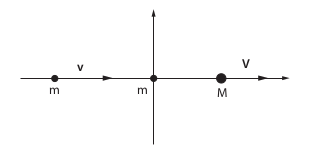
\includegraphics[width=0.8\textwidth]{collision.png}
	\caption{Collision between two particles of mass $m$ resulting in a particle with mass $M$}
	\label{fig:collision}
\end{figure}

Figure \ref{fig:collision} shows a particle with mass $m$ and (relativistic) kinetic energy $V$ in the laboratory frame $S$. The particles is moving towards another particle, with the same mass $m$, which is at rest in $S$.

\subsection{Velocity of First Particle}
Relativistic kinetic energy is given by
\begin{equation}
\label{eq:relkinenergy}
T = (\gamma-1)mc^2.
\end{equation}
Introducing the dimensionless quantity $\alpha = T/mc^2$,
\begin{align*}
\alpha = \frac{T}{mc^2} = \frac{(\gamma - 1)mc^2}{mc^2} &= (\gamma-1) = \frac{1}{\sqrt{1-\frac{v^2}{c^2}}} - 1 \\
\alpha + 1 &= \frac{1}{\sqrt{1-\beta^2}} \\
1 - \beta^2 &= \frac{1}{(\alpha + 1)^2} \\
\beta &= \pm \sqrt{1 - \frac{1}{(\alpha + 1)^2}} \\
v &= \pm c \sqrt{1-(\alpha + 1)^{-2}},
\end{align*}
yields an expression for the velocity of the moving particle.

\subsection{Compound Particle of Perfectly Inelastic Collision}
Assuming that the collision is completely inelastic, they will ``stick together'' after the collision, and form a new compounded particle. The momentum is conserved so that
\begin{equation}
\label{eq:momentumconservation1}
\left(\frac{E_1}{c}, \vb{p}_1 \right) + \left(\frac{E_2}{c}, \vb{p}_2 \right) = \left(\frac{E_3}{c}, \vb{p}_3 \right) ,
\end{equation}
where $E_1 = \gamma(v_1)mc^2$ and $E_2 = \gamma(v_2)mc^2$. Since $v_2 = 0$, $\gamma(v_2) = 1$ and $\vb{p}_2 = \vb{0}$. This gives a relation between the time elements of the four-momenta, which yields the energy of the compounded particle.
\begin{align}
\frac{E_1 + E_2}{c} &= \frac{E_3}{c} \nonumber \\
E_1 + E_2 &= E_3 \nonumber \\
\label{eq:compoundedenergy1}
E = E_3 =  \gamma mc^2 + mc^2 &= (1 + \gamma)mc^2.
\end{align}

Similarly, the momentum of the compounded particle must be
\begin{equation}
P = \vb{p}_3 = \vb{p}_1 = \gamma m\vb{v}_1 = \gamma m v 
\end{equation}

To find the mass $M$ of the compounded particle, one can use the energy-momentum relations
\begin{align*}
E^2 &= (pc)^2 + (Mc^2)^2 \\
\rightarrow M^2c^4 &= E^2 - p^2c^2 =(1+\gamma)^2m^2c^4 - \gamma^2m^2v^2c^2 \\
M^2 &= (1 + 2\gamma + \gamma^2)m^2 - \gamma^2m^2v^2c^{-2} \\
M^2 &= \left[2\gamma + 1 + \gamma^2\left(1-\frac{v^2}{c^2}\right) \right] \\
M^2 & = m^2 (2\gamma + 2) = m^2 2(\gamma + 1)
\end{align*}
\begin{equation}
\label{eq:compoundmass}
M = m \sqrt{2(\gamma + 1)}.
\end{equation}
Notice that in the non-relativistic case, where $v<<c$, $\gamma\to 1$ and $M = 2m$.

The velocity $V$ of the compounded particle can be found by the inverse of the specific Lorentz factor
\begin{equation}
\label{eq:compoundvelocity1}
\gamma_V = \frac{1}{\sqrt{1-\frac{V^2}{c^2}}},\ \rightarrow\ V = c\sqrt{1-\gamma_V^2}.
\end{equation}
Now to find $\gamma(V)$ expressed in some other way. The goal is to find the velocity $V$ as a function of variables that describe the first particle. There are two expressions for the energy of the compounded particle
\begin{align*}
E &= \gamma_V Mc^2 \\
E &= (\gamma + 1)mc^2,
\end{align*}
combining these, and inserting the expression for $M$ from equation \ref{eq:compoundmass} yields
\begin{equation}
\gamma_V m(2(\gamma + 1)) = (\gamma + 1)mc^2 \ \rightarrow \ \gamma_V = \frac{\gamma + 1}{\sqrt{2(\gamma + 1)}}.
\end{equation}
This can now be inserted into \ref{eq:compoundvelocity1}
\begin{equation}
V = c\sqrt{1-\gamma_V^{-2}} = c\sqrt{1-\frac{2}{\gamma+1}} = c\sqrt{\frac{\gamma -1}{\gamma + 1}}.
\end{equation}
This result is a somewhat complicated function of $v$. One way to get a clearer picture of how the velocity of the compounded particle depends on the velocity of the first particle  in the non-relativistic limit would be to do some sort of series expansion\footnote{After a bit of dabbling with Symbolic Python, it appears that $V\approx\frac{1}{2}v$ in the non-relativistic limit.}. 

The initial kinetic energy of the system is $T_1 = (\gamma-1)mc^2$ and the final kinetic energy is $T_2 = E - Mc^2$. The change in kinetic energy is
\begin{align}
\Delta T = T_1 - T_2 	&= (\gamma - 1)mc^2 - (E-Mc^2) \nonumber \\
						&= (\gamma - 1)mc^2 - (\gamma + 1)mc^2 + Mc^2 \nonumber \\
						&= (M - 2m)c^2 \nonumber \\
						&= (\sqrt{2(\gamma + 1)} - 2)mc^2
\end{align}

\subsection{Elastic Collision}
In the rest of this exercise the assumption will be that the particles collide elastically instead. This means that the particles don't form a compounded particle after the collision, but remain the same with no change in their masses. The collision happens in such a way that the particles after the collision make the same angle, $\theta$, with the $x$-axis in the lab frame $S$.

The momentum of the first particle after the collision will be
\begin{equation}
\vb{p}_1 = p_1(\cos\theta, \sin\theta),
\end{equation}
and the momentum of the second particle after the collision will be
\begin{equation}
\vb{p}_2 = p_2(\cos\theta, -\sin\theta).
\end{equation}
Conservation of momentum gives
\begin{equation}
(p_1, 0) = ((p_1 + p_2)\cos\theta,\ (p_1 - p2)\sin\theta).
\end{equation}
The second component gives
\begin{equation}
0 = (p_1 - p_2)\sin\theta \rightarrow 
\begin{cases} 
p_1 = p_2 \\
\sin\theta = 0
\end{cases}
\end{equation}
of which the first case seems more likely, as $\sin\theta = 0$ would imply no angle between the particles at all. Therefore, the magnitude of the momenta of the two particles after the collision must be the same.

The momenta of the particles is the same after the collision,
\begin{equation}
\gamma_1 m v_1 = \gamma_2 m v_2 .
\end{equation}
This means that both velocities and Lorentz factors are the same, ergo
\begin{equation}
E_1 = \gamma_1 mc^2 = \gamma_2 mc^2 = E_2.
\end{equation} 

\subsection{Energy and Momentum}
The energy of the two particles (equation \ref{eq:compoundedenergy1}) should be the same as the combined energy of the two particles, due to conservation of four-momentum.
\begin{equation}
\label{eq:elasticenergy}
E_{Compound} = 2E = (\gamma + 1)mc^2 \rightarrow E = \frac{1}{2}(\gamma + 1)mc^2.
\end{equation}
Making sure the three other elements of the four-momentum vectors are conserved as well gives the momentum of the two particles after the collision
\begin{equation}
\label{eq:elasticmomentum}
\vb{p}_1 = (2\cos\theta, 0) \rightarrow \gamma mv = 2p\cos\theta \rightarrow p = \frac{\gamma mv}{2\cos\theta}
\end{equation}

\subsection{Collision Angle}
Starting with the Energy-momentum relation
\begin{equation*}
E^2 = pc^2 + m^2c^4,
\end{equation*}
inserting energy from \ref{eq:elasticenergy} and momentum from \ref{eq:elasticmomentum} gives
\begin{align*}
\frac{1}{4}(\gamma + 1)^2m^2c^4 &= \frac{\gamma^2m^2v^2c^2}{4\cos^2\theta} + m^2c^4 \\
\frac{\gamma^2m^2v^2c^2}{\cos^2\theta} &= (\gamma +1 )^2m^2c^4 - 4m^2c^4 \\
\frac{\gamma^2m^2v^2c^2}{\cos^2\theta} &= ((\gamma + 1) - 4)m^2c^4 \\
\cos^2\theta &= \frac{v^2}{c^2}\frac{\gamma^2}{(\gamma + 1)^2 - 4}, 
\end{align*}
inserting expressions for $\beta = v/c$ and $\alpha$ from section 2.a gives
\begin{align*}
\cos^2\theta &= \left(1 - \frac{1}{(\alpha +1)^2} \right) \frac{(\alpha + 1)^2}{(\alpha + 2)^2 - 4}\\
			&= \frac{(\alpha + 1)^2 - 1}{(\alpha + 2)^2 -4} = \frac{\alpha^2 + 2\alpha}{\alpha^2 + 4\alpha} = \frac{\alpha + 2}{\alpha + 4} \\
\rightarrow \theta &= \arccos \sqrt{\frac{\alpha + 2}{\alpha + 4}}.
\end{align*}
And lastly,
\begin{equation}
\lim_{\alpha\to 0}\theta = \arccos\frac{1}{\sqrt{2}} = \frac{\pi}{4}
\end{equation}


\end{document}